% -----------------------------------------------
% Template for ISMIR Papers
% 2016 version, based on previous ISMIR templates

% Requirements :
% * 6+1 page length maximum
% * 2MB maximum file size
% * Copyright note must appear in the bottom left corner of first page
% (see conference website for additional details)
% -----------------------------------------------

\documentclass{article}
\usepackage{ismir,amsmath,cite}
\usepackage{graphicx}
\usepackage{color}

% Title.
% ------
\title{Exploiting Harmonics in Convolutional Neural Networks}

% Note: Please do NOT use \thanks or a \footnote in any of the author markup

% Single address
% To use with only one author or several with the same address
% ---------------
%\oneauthor
% {Names should be omitted for double-blind reviewing}
% {Affiliations should be omitted for double-blind reviewing}

% Two addresses
% --------------
%\twoauthors
%  {First author} {School \\ Department}
%  {Second author} {Company \\ Address}

%% To make customize author list in Creative Common license, uncomment and customize the next line
%  \def\authorname{First Author, Second Author} 


% Three addresses
% --------------
\threeauthors
  {First Author} {Affiliation1 \\ {\tt author1@ismir.edu}}
  {Second Author} {\bf Retain these fake authors in\\\bf submission to preserve the formatting}
  {Third Author} {Affiliation3 \\ {\tt author3@ismir.edu}}

%% To make customize author list in Creative Common license, uncomment and customize the next line
%  \def\authorname{First Author, Second Author, Third Author} 

% Four or more addresses
% OR alternative format for large number of co-authors
% ------------
%\multauthor
%{First author$^1$ \hspace{1cm} Second author$^1$ \hspace{1cm} Third author$^2$} { \bfseries{Fourth author$^3$ \hspace{1cm} Fifth author$^2$ \hspace{1cm} Sixth author$^1$}\\
%  $^1$ Department of Computer Science, University , Country\\
%$^2$ International Laboratories, City, Country\\
%$^3$  Company, Address\\
%{\tt\small CorrespondenceAuthor@ismir.edu, PossibleOtherAuthor@ismir.edu}
%}
%\def\authorname{First author, Second author, Third author, Fourth author, Fifth author, Sixth author}


\sloppy % please retain sloppy command for improved formatting

\begin{document}

%
\maketitle
%
\begin{abstract}

% Convnets have rocked MIR
Convolutional neural networks (CNNs), originally pioneered in computer vision, have shown great performance in content-based MIR across a variety of tasks.
% Operate on time-freq reps, which are not images
These models typically operate on time-frequency representations of audio, however, which are statistically distinct from natural images. 
% Sound is harmonic, and model assumptions may not hold.
Convolutional networks exploit statistical regularities in spatial locality, \emph{i.e.}, neighboring pixels. 
While neighboring time-frequency bins also exhibit some regularities, modeling only the local interactions ignores relationships between harmonically related frequencies.
% Make input rep harmonic, does it matter?
Therefore, in an effort to better adapt CNNs to audio, we craft two input representations that aim to exploit this known behavior directly, and determine what effect this has on the learned model.
% How do we do it?
We study these approaches in a large, solo instrument classification task, taking the union of three datasets, and examine how model architecture influences performance.
% What do we find?
%Experimental results show that the use of harmonic convolutions leads to better generalization, faster computation time, and more compact models per unit of performance.
% Closeout
Finally, we provide an open source framework to reproduce both our results and the data used herein.


\end{abstract}
%
\section{Introduction}\label{sec:introduction}

This template includes all the information about formatting manuscripts for the ISMIR \conferenceyear\ Conference.
Please follow these guidelines to give the final proceedings a uniform look.
Most of the required formatting is achieved automatically by using the supplied
style file (\LaTeX) or template (Word).
If you have any questions, please contact the Program Committee
(\texttt{ismir\conferenceyear-papers@ismir.net}).
This template can be downloaded from the ISMIR \conferenceyear\ web site (\texttt{http://ismir\conferenceyear.ismir.net}).
%
\section{Paper Length \& File Size}
Instead of the strict limit of six pages (last used in ISMIR 2014), we adopt 
a ``(6+1)-page policy'' from ISMIR 2015 for ISMIR 2016. This means, the paper may have a 
maximum of 6 pages for technical content including figures and possible references 
with one additional optional 7th page containing only references.
Note that this is a strict requirement. 
\textcolor{red}{The seventh page (if used at all) must
not contain any other material except for references.} 

Paper should be submitted as PDFs and the \textcolor{red}{file size is limited to 2MB}. Please compress images and figures as necessary before submitting.

\section{Page Size}\label{sec:page_size}

The proceedings will be printed on
 \underline{portrait A4-size paper} \underline{(21.0cm x 29.7cm)}.
All material on each page should fit within a rectangle of 17.2cm x 25.2cm,
centered on the page, beginning 2.0cm
from the top of the page and ending with 2.5cm from the bottom.
The left and right margins should be 1.9cm.
The text should be in two 8.2cm columns with a 0.8cm gutter.
All text must be in a two-column format.
Text must be fully justified.

\section{Typeset Text}\label{sec:typeset_text}

\subsection{Normal or Body Text}\label{subsec:body}

Please use a 10pt (point) Times font. Sans-serif or non-proportional fonts
can be used only for special purposes, such as distinguishing source code text.

The first paragraph in each section should not be indented, but all other paragraphs should be.

\subsection{Title and Authors}

The title is 14pt Times, bold, caps, upper case, centered.
Authors' names are omitted when submitting for double-blind reviewing.
The following is for making a camera-ready version.
Authors' names are centered.
The lead author's name is to be listed first (left-most), and the co-authors' names after.
If the addresses for all authors are the same, include the address only once, centered.
If the authors have different addresses, put the addresses, evenly spaced, under each authors' name.

\subsection{First Page Copyright Notice}

Please include the copyright notice exactly as it appears here in the lower left-hand corner of the page.
It is set in 8pt Times.

\subsection{Page Numbering, Headers and Footers}

Do not include headers, footers or page numbers in your submission.
These will be added when the publications are assembled.

\section{First Level Headings}

First level headings are in Times 10pt bold,
centered with 1 line of space above the section head, and 1/2 space below it.
For a section header immediately followed by a subsection header, the space should be merged.

\subsection{Second Level Headings}

Second level headings are in Times 10pt bold, flush left,
with 1 line of space above the section head, and 1/2 space below it.
The first letter of each significant word is capitalized.

\subsubsection{Third and Further Level Headings}

Third level headings are in Times 10pt italic, flush left,
with 1/2 line of space above the section head, and 1/2 space below it.
The first letter of each significant word is capitalized.

Using more than three levels of headings is highly discouraged.

\section{Footnotes and Figures}

\subsection{Footnotes}

Indicate footnotes with a number in the text.\footnote{This is a footnote.}
Use 8pt type for footnotes. Place the footnotes at the bottom of the page on which they appear.
Precede the footnote with a 0.5pt horizontal rule.

\subsection{Figures, Tables and Captions}

All artwork must be centered, neat, clean, and legible.
All lines should be very dark for purposes of reproduction and art work should not be hand-drawn.
The proceedings are not in color, and therefore all figures must make sense in black-and-white form.
Figure and table numbers and captions always appear below the figure.
Leave 1 line space between the figure or table and the caption.
Each figure or table is numbered consecutively. Captions should be Times 10pt.
Place tables/figures in text as close to the reference as possible.
References to tables and figures should be capitalized, for example:
see \figref{fig:example} and \tabref{tab:example}.
Figures and tables may extend across both columns to a maximum width of 17.2cm.

\begin{table}
 \begin{center}
 \begin{tabular}{|l|l|}
  \hline
  String value & Numeric value \\
  \hline
  Hello ISMIR  & \conferenceyear \\
  \hline
 \end{tabular}
\end{center}
 \caption{Table captions should be placed below the table.}
 \label{tab:example}
\end{table}

\begin{figure}
 \centerline{\framebox{
 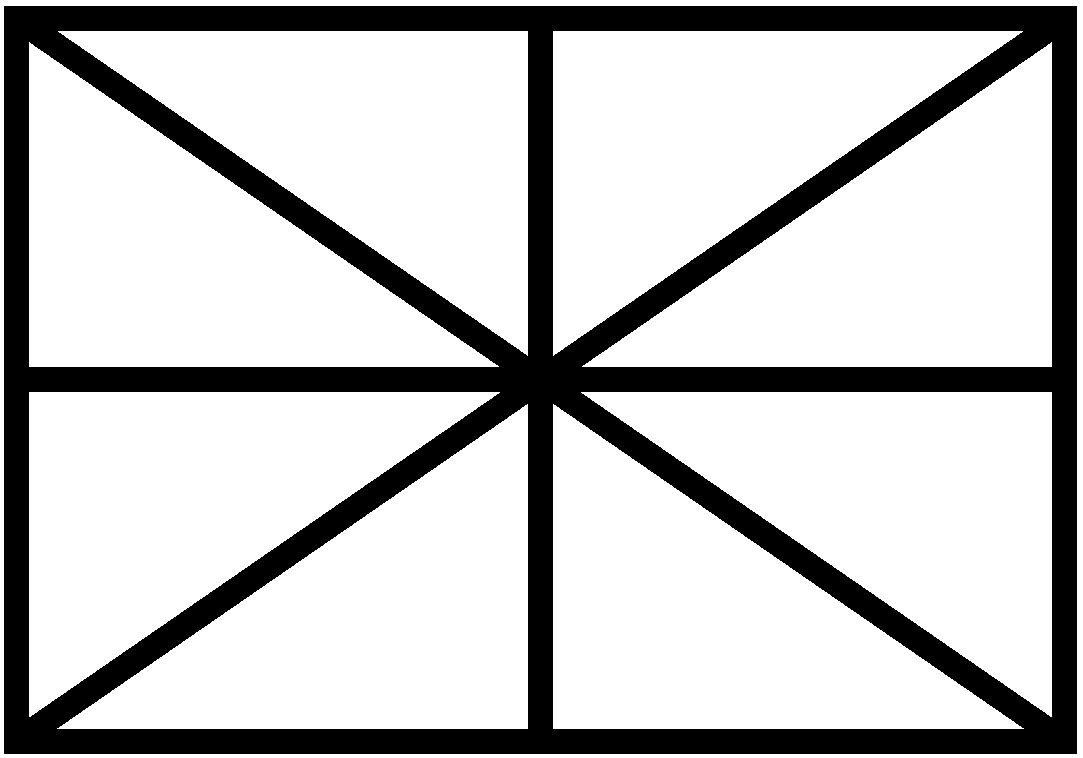
\includegraphics[width=\columnwidth]{figure.png}}}
 \caption{Figure captions should be placed below the figure.}
 \label{fig:example}
\end{figure}

\section{Equations}

Equations should be placed on separate lines and numbered.
The number should be on the right side, in parentheses, as in \eqnref{relativity}.

\begin{equation}\label{relativity}
E=mc^{2}
\end{equation}

\section{Citations}

All bibliographical references should be listed at the end,
inside a section named ``REFERENCES,'' numbered and in alphabetical order.
All references listed should be cited in the text.
When referring to a document, type the number in square brackets
\cite{Author:00}, or for a range \cite{Author:00,Someone:10,Someone:04}.

% For bibtex users:
\bibliography{references}

% For non bibtex users:
%\begin{thebibliography}{citations}
%
%\bibitem {Author:00}
%E. Author.
%``The Title of the Conference Paper,''
%{\it Proceedings of the International Symposium
%on Music Information Retrieval}, pp.~000--111, 2000.
%
%\bibitem{Someone:10}
%A. Someone, B. Someone, and C. Someone.
%``The Title of the Journal Paper,''
%{\it Journal of New Music Research},
%Vol.~A, No.~B, pp.~111--222, 2010.
%
%\bibitem{Someone:04} X. Someone and Y. Someone. {\it Title of the Book},
%    Editorial Acme, Porto, 2012.
%
%\end{thebibliography}

\end{document}
